\documentclass[14pt]{extreport}

\usepackage[utf8]{inputenc}
\usepackage[T2A]{fontenc}
\usepackage[english,ukrainian]{babel}
\usepackage{tempora}

\usepackage{float}
\usepackage{caption}
\captionsetup[table]{justification=raggedleft, singlelinecheck=false, labelsep=period}
\captionsetup[figure]{labelsep=space}
\usepackage{graphicx}
\graphicspath{ {./pictures} }
\usepackage{listings}
\lstset{breaklines=true,showstringspaces=false}
\linespread{1.5}
\setlength{\parskip}{0pt}
\usepackage{indentfirst}

\usepackage[a4paper,top=20mm,bottom=20mm,left=25mm,right=10mm]{geometry}

\usepackage{fancyhdr}
\fancypagestyle{plain}{
  \pagestyle{myheadings}
}
\pagestyle{myheadings}

\usepackage{titlesec}
\titleformat{\chapter}{\centering\bfseries\MakeUppercase}{}{1pc}{}
\titleformat{\section}{\centering\bfseries\MakeUppercase}{}{1pc}{}
\titleformat{\subsection}{\bfseries}{}{1pc}{}
\titleformat{\subsubsection}{\bfseries}{}{1pc}{}
% \titleformat{\paragraph}{\bfseries}{}{}{}

\titlespacing*{\chapter}{0pt}{10mm}{14pt}
\titlespacing*{\section}{\parindent}{14pt}{0pt}
\titlespacing*{\subsection}{\parindent}{0pt}{0pt}
\titlespacing*{\subsubsection}{\parindent}{0pt}{0pt}
\titlespacing*{\paragraph}{\parindent}{0pt}{7pt}

\usepackage{enumitem}
\setlist{nolistsep}

\usepackage{hyperref}
\def\UrlBreaks{\do\/\do-}
\makeatletter
\renewcommand{\thesection}{\@arabic\c@section}
\makeatother

\begin{document}

\setcounter{page}{2}
\tableofcontents
\newpage

\section{Короткий опис бази практики}

\subsection{Фокусні галузі}
Основними напрямками діяльності бази практики є розробка програмного забезпечення з використанням блокчейн-технологій, створення децентралізованих застосунків (dApp), надання консалтингових послуг у сфері Web3 та смарт-контрактів, а також дослідження новітніх підходів до забезпечення безпечної взаємодії користувачів у розподілених системах.

\subsection{Технічні й програмні засоби}
У роботі використовуються такі технічні та програмні засоби, як мова програмування Rust для розробки смарт-контрактів, інструменти Solana CLI, Solana SDK та Anchor Framework. Клієнтська частина розробляється на основі Wasm або Web3 бібліотек. Для контролю версій застосовуються Git та GitHub, а серед середовищ розробки використовуються VS Code та Neovim.

\subsection{Характер робіт, пов’язаних із застосуванням ІТ}
Характер робіт передбачає створення прикладного програмного забезпечення з використанням сучасних середовищ розробки та засобів командного рядка. Важливим аспектом є робота з системами контролю версій для ефективного керування кодовою базою, а також налаштування локального середовища розробки та тестування. Студенти будуть залучені до роботи з документацією, технічними специфікаціями та вимогами до програмного забезпечення, інтеграції криптографічних механізмів підпису й перевірки транзакцій, а також до формування технічної звітності та проектної документації.

\section{Завдання, отримане на базі практики}

\begin{enumerate}
	\item Ознайомитись із основами технології блокчейн та принципами її застосування.
	\item Вивчити екосистему Solana та її програмну модель для створення смарт-контрактів.
	\item Створити простий смарт-контракт (on-chain програму).
	\item Розробити клієнтську частину для взаємодії зі смарт-контрактом.
	\item Провести локальне тестування розробленої системи за допомогою тестової мережі Solana.
	\item Забезпечити базову перевірку автентичності користувачів шляхом підпису транзакцій гаманцем.
\end{enumerate}

\section{Результати виконання завдання на базі практики}

У процесі проходження практики було проведено аналіз технології блокчейн, розглянуто архітектуру та принципи роботи мережі Solana, досліджено інструменти розробки смарт-контрактів, виконано програмну реалізацію прикладного застосунку для роботи з блокчейном, а також здійснено інтеграцію смарт-контракту з клієнтською частиною.

\subsection{Теоретичні основи}

На першому етапі розглянуто теоретичні засади блокчейн-технологій, включно з наступними поняттями:
\begin{itemize}
    \item Розподілений реєстр;
    \item Консенсусні алгоритми (Proof of Work, Proof of Stake, Proof of History);
    \item Публічні та приватні ключі, криптографія;
    \item Смарт-контракти.
\end{itemize}

Особливу увагу приділено мережі Solana, яка забезпечує високу пропускну здатність за рахунок унікального механізму \textbf{Proof of History}. Розглянуто архітектуру валідаторів, транзакцій, акаунтів, смарт-контрактів (програм) та системи розподіленої пам’яті.

\subsection{Інструменти розробки}

Для створення та розгортання смарт-контрактів було використано такі інструменти:
\begin{itemize}
    \item \textbf{Rust} — основна мова програмування;
    \item \textbf{Anchor} — фреймворк для спрощення розробки програм під Solana;
    \item \textbf{Solana CLI} — інтерфейс командного рядка для управління акаунтами та розгортання програм;
    \item \textbf{Phantom Wallet} — браузерний гаманець для взаємодії з мережею Solana.
\end{itemize}

\subsection{Програмна реалізація}

Під час практики було створено смарт-контракт лічильника, що містить функціонал:
\begin{itemize}
    \item Ініціалізація об’єкта рахунку;
    \item Збільшення значення лічильника;
    \item Зменшення значення лічильника з перевіркою суми.
\end{itemize}

Смарт-контракт реалізовано за допомогою Anchor. Наведено приклад структури даних:

\begin{verbatim}
#[account]
pub struct Counter {
    pub count: u64,
}
\end{verbatim}

Та приклад функції:

\begin{verbatim}
pub fn increment(ctx: Context<Increment>) -> Result<()> {
    let counter = &mut ctx.accounts.counter;
    counter.count += 1;
    Ok(())
}
\end{verbatim}

\subsection{Графічний інтерфейс}

Було створено клієнтську частину за допомогою фреймворку React, яка дозволяє:
\begin{itemize}
    \item Авторизацію через Phantom Wallet;
    \item Ініціалізацію лічильника;
    \item Інтерактивне збільшення/зменшення значення;
    \item Виведення результату на екран.
\end{itemize}

Для взаємодії з Solana-програмою у браузері використовувалась бібліотека \texttt{@solana/web3.js}.

\subsection{Тестування та демонстрація}

Тестування проводилось у локальному кластері Solana (test validator). Здійснено розгортання програми, перевірку транзакцій, підписування з Phantom Wallet, аналіз змін значення лічильника після виконання інструкцій.

\begin{figure}[H]
    \centering
    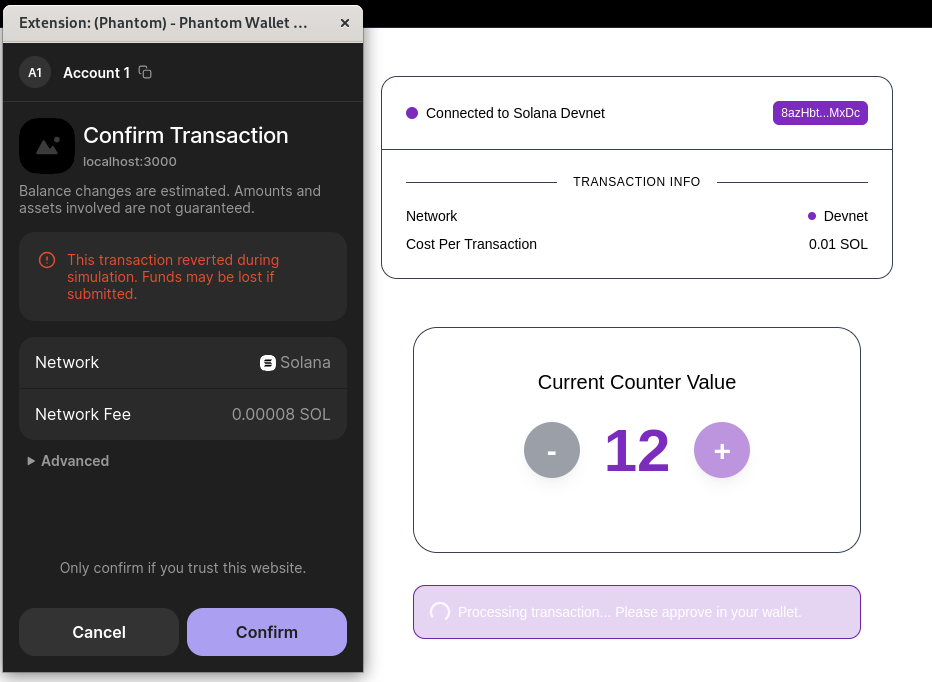
\includegraphics[width=0.5\textwidth]{2}
    \caption{Інтерфейс авторизації через Phantom}
\end{figure}

\begin{figure}[H]
    \centering
    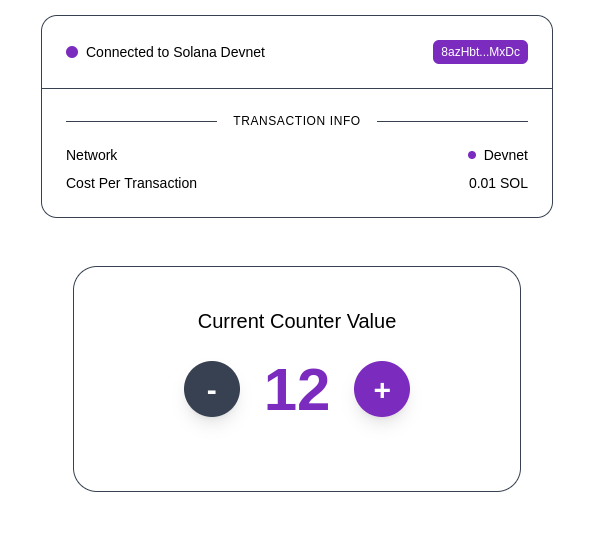
\includegraphics[width=0.5\textwidth]{1}
    \caption{Інтерфейс керування лічильником}
\end{figure}

\subsection{Висновки}

Результатом практики стало створення функціонального децентралізованого застосунку на базі мережі Solana. Набуто практичні навички роботи з Anchor, Rust, React, смарт-контрактами, а також досвід інтеграції блокчейн-функціоналу у вебінтерфейс. Практика дозволила сформувати цілісне уявлення про розробку та розгортання DApp від ідеї до реалізації.


\section{Завдання стосовно дипломного проекту}

\begin{enumerate}
    \item Підготувати оглядовий розділ БКР, який включатиме теоретичні основи технології блокчейн та екосистеми Solana.
    \item Сформувати постановочний розділ БКР, де буде обґрунтовано актуальність розробки, визначено мету і завдання дослідження, а також описано предмет і об'єкт розробки.
    \item Розробити проектний розділ БКР, який детально описуватиме розроблений смарт-контракт та клієнтську частину, включаючи їхню архітектуру, функціональність та процес тестування.
\end{enumerate}

\section{Опис проведених робіт стосовно БКР}

У межах переддипломної практики було підготовлено оглядовий, постановочний і проєктний розділи бакалаврської кваліфікаційної роботи, що стали основою для подальшої розробки системи електронного голосування. В оглядовому розділі проаналізовано наукові публікації, сучасні технології та рішення у сфері е-голосування, зокрема блокчейн, алгоритми консенсусу (PoW, PoS, PoH), криптографічні методи та переваги/недоліки централізованих і децентралізованих систем. Це дало змогу визначити актуальні напрями дослідження.

У постановочному розділі обґрунтовано доцільність використання блокчейн-платформи Solana та мови Rust, сформульовано мету, завдання й вимоги до системи. У проєктному розділі описано функціональні можливості системи, ролі користувачів та основні характеристики продукту.


\section*{Висновки}
\addcontentsline{toc}{section}{Висновки про отримані результати}

У ході практики вивчено теоретичні основи блокчейн та екосистему Solana. Розроблено простий смарт-контракт і клієнтську частину для взаємодії з ним, включаючи базову автентифікацію користувачів через криптогаманець. Проведено локальне тестування розробленої системи.

Також виконано значний обсяг робіт для бакалаврської кваліфікаційної роботи, включаючи підготовку оглядового, постановочного та проектного розділів, що закладають теоретичну та методологічну основу для дослідження системи електронного голосування на базі блокчейн-технологій.

\newpage
\section*{Список використаних джерел}
\addcontentsline{toc}{section}{Список використаних джерел}

\begin{enumerate}
\item Nakamoto, S. (2008). Bitcoin: A Peer-to-Peer Electronic Cash System. (Електронний ресурс). Посилання: \href{https://bitcoin.org/bitcoin.pdf}{https://bitcoin.org/bitcoin.pdf}
\item Solana Foundation. (n.d.). Solana Documentation. (Електронний ресурс). Посилання: \href{https://docs.solana.com/}{https://docs.solana.com/}
\item Anchor Framework. (n.d.). Anchor Book. (Електронний ресурс). Посилання: \href{https://www.anchor-lang.com/book}{https://www.anchor-lang.com/book}
\item Phantom Wallet. (n.d.). Phantom - Solana Wallet. (Електронний ресурс). Посилання: \href{https://phantom.app/}{https://phantom.app/}

\end{enumerate}

\newpage

\section*{Додаток А.\hspace{0.5em} Код програми}
\addcontentsline{toc}{section}{Додатки}
{\small
\begin{lstlisting}
use anchor_lang::prelude::*;
use anchor_lang::system_program;

declare_id!("DGmJsbjsife1p3QoueUruomvJXLaYXMwqEFgE4bV4xrg");

#[program]
mod solana_counter {
    use super::*;

    pub fn initialize(ctx: Context<Initialize>) -> Result<()> {
        let counter = &mut ctx.accounts.counter;
        counter.count = 0;
        Ok(())
    }

    pub fn increment(ctx: Context<Increment>, payment: u64) -> Result<()> {
        let counter_account_info = ctx.accounts.counter.to_account_info();
        let user = &ctx.accounts.user;

        const MINIMUM_PAYMENT: u64 = 10_000_000; // 0.01 SOL dalam lamports
        require!(payment >= MINIMUM_PAYMENT, ErrorCode::InsufficientPayment);

        let cpi_context = CpiContext::new(
            ctx.accounts.system_program.to_account_info(),
            system_program::Transfer {
                from: user.to_account_info(),
                to: counter_account_info,
            },
        );
        system_program::transfer(cpi_context, payment)?;

        let counter = &mut ctx.accounts.counter;
        counter.count += 1;
        Ok(())
    }

    pub fn decrement(ctx: Context<Decrement>, payment: u64) -> Result<()> {
        let counter_account_info = ctx.accounts.counter.to_account_info();
        let user = &ctx.accounts.user;

        const MINIMUM_PAYMENT: u64 = 10_000_000; // 0.01 SOL dalam lamports
        require!(payment >= MINIMUM_PAYMENT, ErrorCode::InsufficientPayment);

        let cpi_context = CpiContext::new(
            ctx.accounts.system_program.to_account_info(),
            system_program::Transfer {
                from: user.to_account_info(),
                to: counter_account_info,
            },
        );
        system_program::transfer(cpi_context, payment)?;

        let counter = &mut ctx.accounts.counter;
        require!(counter.count > 0, ErrorCode::CounterUnderflow);
        counter.count -= 1;
        Ok(())
    }
}

#[derive(Accounts)]
pub struct Initialize<'info> {
    #[account(
        init,
        payer = user,
        space = 8 + 8, // Discriminator (8) + u64 (8)
        seeds = [b"counter"],
        bump
    )]
    pub counter: Account<'info, Counter>,
    #[account(mut)]
    pub user: Signer<'info>,
    pub system_program: Program<'info, System>,
}

#[derive(Accounts)]
pub struct Increment<'info> {
    #[account(
        mut,
        seeds = [b"counter"],
        bump
    )]
    pub counter: Account<'info, Counter>,
    #[account(mut)]
    pub user: Signer<'info>,
    pub system_program: Program<'info, System>,
}

#[derive(Accounts)]
pub struct Decrement<'info> {
    #[account(
        mut,
        seeds = [b"counter"],
        bump
    )]
    pub counter: Account<'info, Counter>,
    #[account(mut)]
    pub user: Signer<'info>,
    pub system_program: Program<'info, System>,
}

#[account]
pub struct Counter {
    pub count: u64,
}

#[error_code]
pub enum ErrorCode {
    #[msg("Payment is insufficient")]
    InsufficientPayment,
    #[msg("Counter cannot go below zero")]
    CounterUnderflow,
}
\end{lstlisting}
}

\end{document}
